\chapter{Sistema Mecatrônico}\label{cap:Metodologia}

De maneira geral, a estrutura do robô possui forma retangular com duas rodas. As rodas são acopladas de forma que fiquem paralelas uma a outra. A estrutura pode ser comparada como uma estante, no qual o mesmo foi projetado para três e em cada uma delas estão alguns componentes.  A Figura (\ref{fig:EstruturaRealVisaoFrontalLateral}) mostra a vista isométrica da estrutura.
\begin{figure}[H]
    \centering
    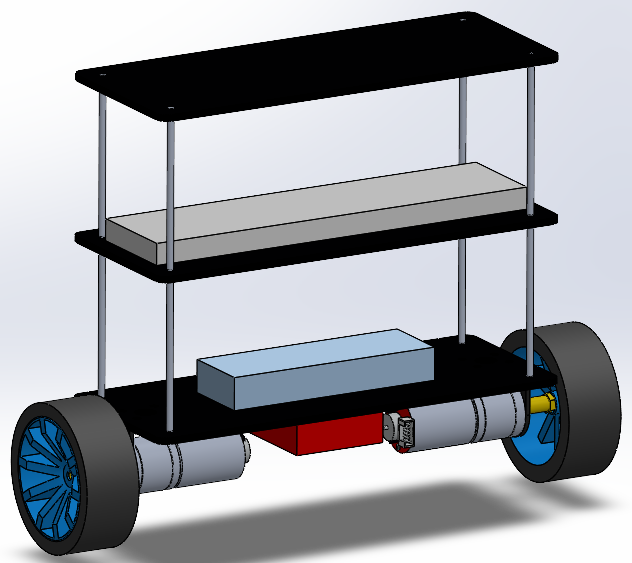
\includegraphics[scale=0.6]{Metodologia/Pendulo_3D.PNG}
    \caption{Estrutura real do pêndulo na visão frontal e lateral.}
    \label{fig:EstruturaRealVisaoFrontalLateral}
\end{figure}

\section{Estrutura Adotada}\label{sec:EstruturaCAD}

A estrutura do pêndulo consiste em quatro barras rosqueadas que serve para sustentar as prateleiras em seus devidos lugares. O material utilizado para fazer as bases do pêndulo foi o ACM. Foi adotado uma altura de 200 $mm$ para a planta medindo do chão ao topo, a largura de 80 $mm$ que é o padrão das placas com uma espessura de 3 $mm$. 
Os componentes do sistema foram distribuídos em cada andar. Na parte inferior da primeira estante ou no ponto mais próximo ao solo temos o \textit{driver} dos motores e os motores propriamente dito. Contudo, foi necessário a utilização de um suporte que fixasse os motores a base. Já no segundo andar ou na segunda prateleira, estão o microprocessador Arduino Nano e o sensor que capturará o ângulo de inclinação da planta. Por fim, para deixar o centro de massa um pouco mais distante do eixo de referência que passa entre os motores, posicionou-se a bateria na última placa. Em muitas literaturas aconselha-se adotar esse tipo de estratégia para facilitar o controle do pêndulo invertido.

\subsection{Parâmetros Mecânicos da Estrutura}

A Tabela (\ref{tab:ParametroEstrutura}) apresenta os parâmetros mecânicos da estrutura do pêndulo bem como seus respectivos valores. Tais parâmetros foram medidos ou mesmo calculados como mostra o Apêndice ().
\begin{table}[!htb]
\centering
\caption{Parâmetros mecânicos obtidos através de medições práticas e via cálculos.}
\label{tab:ParametroEstrutura}
\begin{tabular}{@{}cccc@{}}
\toprule
\textbf{Descrição da grandeza} & \multicolumn{1}{l}{\textbf{Variável}} & \textbf{Valor Nominal} & \textbf{Unidade de medida} \\ \midrule
Momento de Inércia do Pêndulo           & $J_p$         & 0.00530429    & $kg.m^2$    \\
Momento de Inércia das Rodas            & $J_w$         & 0.00005013    & $kg.m^2$    \\
Massa total da planta física            & $m$           & 0.7740        & $kg$      \\
Massa do pêndulo s/rodas                & $M_{p}$       & 0.7120        & $kg$      \\
Massa de duas rodas                     & $M_{r}$       & 0.0620        & $kg$      \\
Altura do centro de massa ao eixo    & $z_{cm}$      & 0.0836        & $m$         \\
Raio externo das rodas                  & $r_{ext}$     & 0.0315        & $m$         \\
Raio interno das rodas                  & $r_{int}$     & 0.0250        & $m$         \\
Distância eixo até o conjunto-placa 1   & $d_{h1}$      & 0.0150        & $m$       \\
Distância eixo até o conjunto-placa 2   & $d_{h2}$      & 0.120         & $m$       \\
Distância eixo até o conjunto-placa 3   & $d_{h3}$      & 0.180         & $m$       \\
Distância do chão até o topo            & $H$           & 0.200         & $m$       \\
Largura dos conjuntos-placa             & $W$           & 0.080         & $m$       \\
Resistência de armadura do motor        & $R$           & 0.91          & $\Omega$  \\
\bottomrule
\end{tabular}
\end{table}

\section{Instrumentação}

No momento em que se inicia o planejamento de um projeto de engenharia, é de suma importância
realizar a listagem dos recursos que serão utilizados, bem como a justificativa de cada. Desta
forma, segue abaixo a listagem dos \textit{softwares} e materiais que foram ordenados da seguinte maneira: atuadores, transdutor de orientação e eletrônica.

\subsection{Arduino Nano}

O Arduino Nano é um microcontrolador de baixo custo e de alta performance. Essa placa será responsável por realizar o controle do sistema, fazer a leitura dos sinais do sensor e enviar os sinais de controle para o atuador. A placa pode ser vista na Figura (\ref{fig:ArduinoNano}).
\begin{figure}[H]
    \centering
    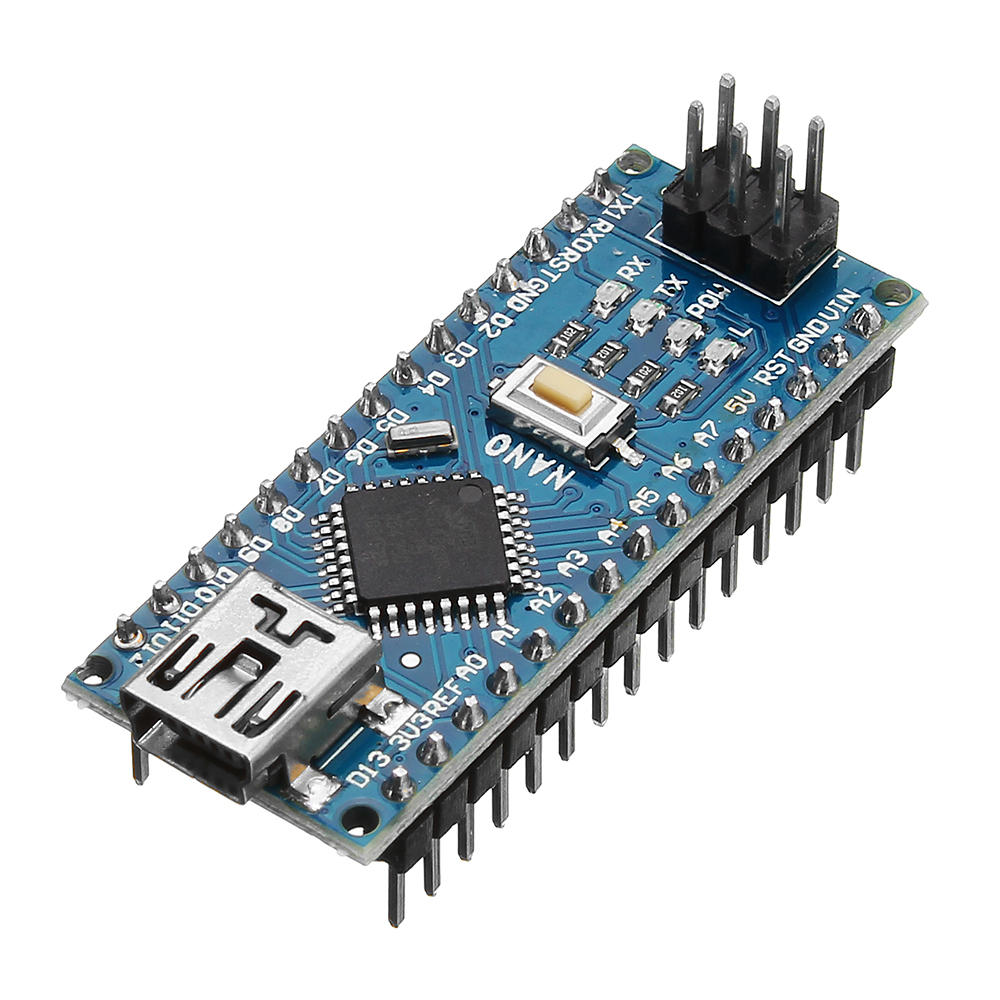
\includegraphics[scale=0.15]{Metodologia/arduinoNano}
    \caption{Visão da placa responsável pela leitura dos sinais do sensor e processamento dos sinais de controle.}
    \label{fig:ArduinoNano}
\end{figure}

A decisão da utilização dessa placa ao invés de outro microcontrolador seu deu pelo fato de que a mesma conseguiria suprir os requisitos para o projeto, como a quantidade mínima de pinos PWM e digitais e a capacidade de processamento dos dados. A partir do \textit{datasheet} da placa, é possível conhecer as características principais que a compõe, como visto abaixo.
\begin{table}[!htb]\label{tab:CaracteristicaArduinoNano}
\centering
\caption{Dados do fabricante sobre a placa Arduino Nano.}
\begin{tabular}{lc}
\hline
\textbf{Descrição}               & \textbf{Valores Nominais}    \\ \hline
Chip                             & ATmega328P – 8 bit AVR       \\
Tensão de Operação               & 5 $V_{cc}$                   \\
Tensão de Alimentação $(V_{in})$ & 7$\sim$12 $V_{cc}$             \\
Pinos Digitais                   & 14 (D0 - D13)                \\
Pinos Digitais PWM               & D3, D5, D6, D9, D11 (8 bit)  \\ 
Pinos Analógicos                 & 8 (A0 - A7)                  \\
Corrente Máxima p/Pino           & 40 $mA$                      \\
Memória Flash                    & 32 $kB$                      \\
Clock                            & 16 $MHz$                     \\ \hline
\end{tabular}
\end{table}

\subsection{Driver Motor CC}

A Figura (\ref{fig:PonteH}) apresenta o \textit{driver} do motor CC que será utilizado, a Ponte H L298N. Com essa placa será possível realizar o controle de sentido de giro e realizar o controle da velocidade dos dois motores por meio de sinais PWM ($\textit{Pulse Width Modulation}$).
\begin{figure}[H]
    \centering
    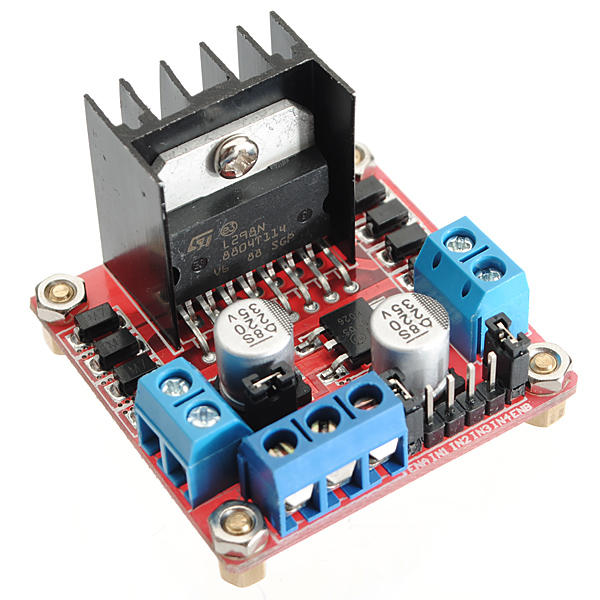
\includegraphics[scale=1]{Metodologia/L298N}
    \caption{Visualização comercial do \textit{driver} Ponte H L298N.}
    \label{fig:PonteH}
\end{figure}

Todas as características dessa placa se encontram na folha de dados do fabricante e algumas das mais importantes a serem consideradas podem ser vistas na Tabela (\ref{tab:CaracteristicaMPU}).
\begin{table}[!htb]\label{tab:CaracteristicaMPU}
\centering
\caption{Parâmetros mecânicos da estrutura.}
\begin{tabular}{lc}
\hline
\textbf{Descrição}              & \textbf{Valores Nominais}   \\ \hline
Tensão de Operação              & 4$\sim$35 $V_{cc}$          \\
Tensão Lógica                   & 5$V$                        \\
Corrente de Operação Máxima     & 2$A$ por canal              \\
Corrente Lógica                 & 0$\sim$36 $mA$              \\
Dimensões (C$\times$L$\times$A) & 43$\times$43$\times$27 $mm$ \\ \hline
\end{tabular}
\end{table}

Como mencionado, com essa placa realiza-se duas coisas importantes, mudança no sentido de giro e a alteração da velocidade dos motores. O primeiro caso é realizado mudando o sentido da corrente, pois os motores CC giram a partir de um campo magnético que é provocado por uma corrente que passa em suas bobinas. Já no segundo caso temos a variação de velocidade por meio do sinal PWM, na qual a tensão de saída que chegará nos terminais do motor será uma tensão média que sempre dependerá do ciclo de trabalho daquele instante.

Como mencionado, com essa placa realiza-se duas coisas importantes, mudança no sentido de giro e alteração da velocidade dos motores. O primeiro caso é realizado mudando o sentido da corrente, pois os motores CC giram a partir de um campo magnético que é provocado por uma corrente que passa em suas bobinas.

Para controlar a velocidade do motor, é necessário recorrer ao PWM, que nada mais é do que uma técnica que obtém resultados analógicos por meio digitais. A técnica consiste em ondas quadradas de alta frequência das quais é possível controlar o percentual de tensão que é aplicado aos motores. Para realizar isto, basta controlar o tempo que deseja manter a saída em 1 (ou ligado) e o em 0 (ou desligado). Esse tempo em nível alto é chamado de $\textit{Duty Cicle}$ e ao utilizar desse recurso, o valor médio de tensão aplicado aos terminais do motor será alterado. 

A partir da Figura (\ref{fig:PWM}), é possível obter a equação do $\textit{Duty Cicle}$ (DC) e da tensão média que será de fato o valor aplicado aos motores.
\begin{equation}
    \begin{array}{cc}
         &  DC = \dfrac{DT}{T}\\[20pt]
         &  U_{medio} = U_{max}(DC)
    \end{array}{}
\end{equation}{}

\begin{figure}[!htb]
    \centering
    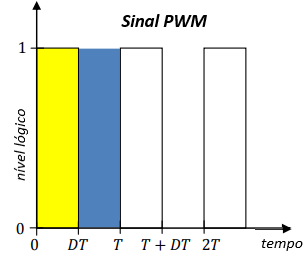
\includegraphics[scale=1]{Metodologia/PWM}
    \caption{Representação de um sinal PWM.}
    \label{fig:PWM}
\end{figure}

\subsection{Atuador}

A Figura \ref{fig:KitMotor} mostra o atuador da planta escolhido juntamente com seus componentes complementares. O motor é responsável por receber o sinal do controle e transformar em tração, movimentando assim o pêndulo.
\begin{figure}[!htb]
    \centering
    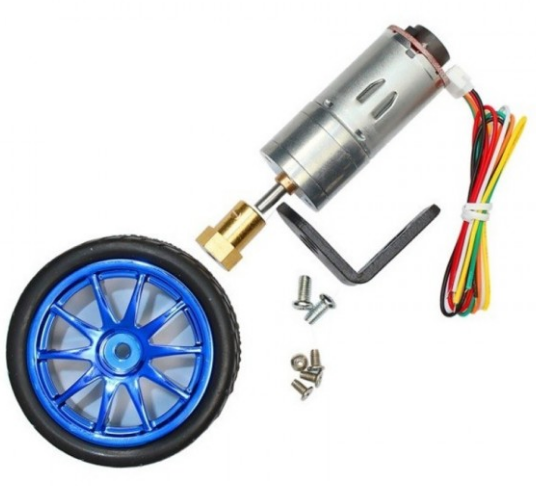
\includegraphics[scale=0.45]{Metodologia/KitMotor}
    \caption{Conjunto completo do atuador composto por motor, roda, suporte de acoplamento da roda ao motor, suporte de acoplamento do motor à base e parafusos.}
    \label{fig:KitMotor}
\end{figure}

\subsubsection{Motores}

O motor escolhido em questão opera com uma tensão de 6V contínuo com uma taxa de redução de 34:1 que faz com tenha pouco \textit{backlash}. Possui encoder de quadratura acoplado na parte anterior de resolução de 11 pulsos por resolução no eixo do motor, que corresponde a 341.2 pulsos por resolução na saída após a caixa de redução. Normalmente, motores pequenos e de baixo preços costumam não possuir uma folha de dados completa e, portanto, as constantes dos mesmo são desconhecidas. Mas nas especificações disponíveis há a tensão nominal ou de operação, velocidade e corrente sem carga, torque, velocidade, potência e corrente em máxima eficiência. Como o motor é de polos é possível encontrar resistência de armadura de forma direta medindo por meio de um multímetro seus terminais. Neste dois casos desconsidera indutância por se tratar de um valor muito pequeno e sua influência será praticamente nula \cite{Sundin:12}.

\begin{table}[!htb]\label{tab:ParametrosDatasheetMotor}
\centering
\caption{Dados do fabricante em relação ao motor.}
\begin{tabular}{lc}
\hline
\textbf{Condições}       & \textbf{Valores Nominais}              \\ \hline

Tensão Operação          & 6 $V_{cc}$                           \\
Resistência de armadura  & 8 $\Omega$                           \\
Velocidade Sem Carga     & 210$RPM$ (0.13$A$)                       \\
Eixo Travado             & 0.980665$Nm$ (3.2$A$)                    \\
Máxima Eficiência        & 0.196133$Nm$ / 170$RPM$ / 2.0$W$ / 0.60$A$     \\
Máxima Potência          & 0.509946$Nm$ / 110$RPM$ / 3.1$W$ / 1.10$A$ \\
Taxa de Redução          & 34:1                                 \\
 
\hline
\end{tabular}
\end{table}

\subsubsection{Rodas}

O conjunto roda e pneus utilizados possuem dimensão de 65$\times$25$mm$. As rodas foram escolhidas desse tamanho por considerar que as mesmas atendem a velocidade angular do motor e a velocidade desejada para o sistema. Por sua vez, a roda é fabricada por um tipo de plástico azul brilhante e os pneus por borracha. O conjunto é acoplado ao motor através de um suporte e fixado por um parafuso bem no centro da roda. O conjunto será aproximado por por um anel para o cálculo do momento de inércia e não por um cilindro maciço já que as rodas é vazada e possuem alguns rasgos.
\begin{table}[!htb]\label{tab:ParametrosRoda}
\centering
\caption{Parâmetros da roda obtidos experimentalmente.}
\begin{tabular}{@{}cccc@{}}
\toprule
\textbf{Parâmetro} &\textbf{Valor Nominal} &\textbf{Unidade} &\textbf{Descrição}       \\ \midrule

\textbf{$M_r$}     & 0.0310         & $kg$            & Massa de cada roda       \\
\textbf{$r_{1}$}       & 0.0250         & $m$             & Raio interno da roda             \\
\textbf{$r_{2}$}       & 0.0315         & $m$             & Raio externo da roda             \\
\bottomrule
\end{tabular}
\end{table}

\subsection{Transdutor de Orientação}

Essa $\textit{shield}$ possui dois sensores, acelerômetro e giroscópio, dos quais serão fundidos a fim de obter uma melhor precisão da medição da orientação da estrutura do pêndulo. A Figura (\ref{fig:MPU6050}) apresenta a placa física e um modelo que representa todos os 6 eixos, 3 para o acelerômetro e 3 para o giroscópio, o que faz com a mesma possua 6 graus de liberdade ($\textit{6DOF}$). 
\begin{figure}[H]
    \centering
    \subfigure[\label{PlacaMPU6050}]{
    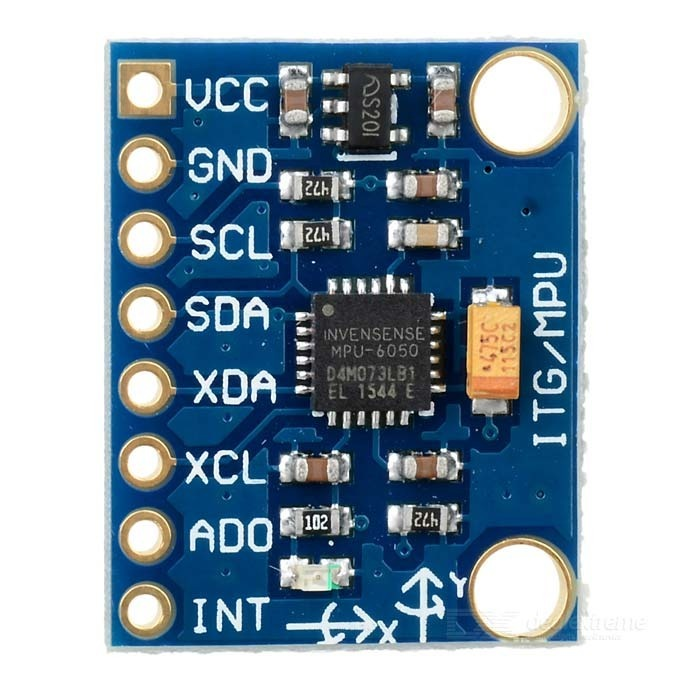
\includegraphics[scale=0.13]{Metodologia/MPU6050}}
    \subfigure[\label{MPUEixos}]{
    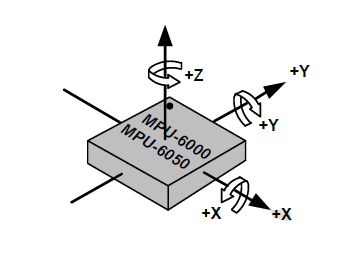
\includegraphics[scale=0.47]{Metodologia/IMUEixos}}
    \caption{A placa comercial é vista em (a) e os detalhes dos eixos do sensor de orientação utilizado para medição da inclinação do robô é visto em (b).}
    \label{fig:MPU6050}
\end{figure}

A partir do \textit{datasheet} da placa algumas características podem ser obtidas como visto na Tabela (\ref{tab:ParametrosPlacaMPU6050}).
\begin{table}[!htb]
\centering
\caption{Principais características da placa MPU6050 \citep{MPU6050}.}
\label{tab:ParametrosPlacaMPU6050}
\begin{tabular}{@{}lc@{}}
    \toprule
    \textbf{Descrição}              & \textbf{Valores}             \\ 
    \midrule
    Modelo                          & GY-521                        \\
    Tensão de Operação              & 3 $\sim$ 5 $V_{cc}$           \\
    Conversor ADC                   & 16 $bits$                     \\
    Comunicação                     & $I^2C$                        \\ 
    Tempo de Acomodação             & 10 $ms$                       \\
    Dimensões (C$\times$L$\times$A) & 21$\times$17$\times$3 $mm$    \\ 
    \bottomrule
\end{tabular}
\end{table}

\subsubsection{Acelerômetro}
O acelerômetro é um equipamento que é utilizado para mensurar sua aceleração própria. A aceleração própria é diferente daquela estabelecida através da relação entre velocidade e tempo. Sendo que esta considera a sensação de peso medida em um dado referencial. Quando considera-se o acelerômetro colocado em uma superfície plana, a medição será de aproximadamente $9.81 m/s^2$. Na maioria dos casos, a aceleração é medida em força g, que é basicamente a aceleração sentida como peso. A Figura (\ref{fig:InclinacaoAcelMPU}) mostra a inclinação de algum objeto utilizando dois eixos. 
\begin{figure}[H]
    \centering
    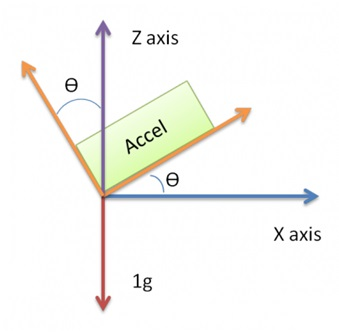
\includegraphics[scale=0.7]{Metodologia/Acelerometro}
    \caption{Detalhamento de forma gráfica dos 3 eixos do acelerômetro.}
    \label{fig:InclinacaoAcelMPU}
\end{figure}

A medição da orientação pode ser feita de três maneiras: utilizando apenas um eixo, dois e três eixos. A forma mais simples é a primeira, porém a mais eficiente em termos de precisão é a última. As equações são mostradas logo abaixo:
\begin{equation}
    \begin{array}{ccc}
         &  \theta = \sin^{-1}(x) \\[10pt]
         &  \theta = \arctan \left(\dfrac{x}{z}\right)  \\[10pt]
         &  \theta = \arctan \left(\dfrac{x}{\sqrt{z^2+y^2}}\right)
    \end{array}{}
\end{equation}{}

\subsubsection{Giroscópio}
O giroscópio por sua vez, é um dispositivo utilizado para manter ou medir a orientação. Um giroscópio mecânico normalmente consiste de um disco rotativo, em que os eixos ligados a ele são capazes de se deslocarem livremente em qualquer orientação. 

O valor lido da MPU6050 sem nenhum tratamento pode ser chamado de valor bruto já que não representa nenhuma grandeza física e para realizar a conversão para um valor usual, é necessário saber/configurar o quão rápido o sensor está girando em graus por segundo $(dps)$. A Tabela (\ref{tab:ParamGiroMPU}), com conteúdo encontrado no $\textit{datasheet}$ do fabricante, relaciona cada velocidade de giro do sensor com a sua sensibilidade, sendo que essas constantes são chamadas de ganho e devem ser divididas por 1000.
\begin{table}[!htb]
    \centering
    \caption{Parâmetros do giroscópio: velocidade de giro e nível de sensibilidade.}
    \label{tab:ParamGiroMPU}
    \begin{tabular}{@{}cc@{}}
        \toprule
        \textbf{Faixa ($^{\circ}$/s)} & \textbf{Sensibilidade LSB/($^{\circ}$/s)} \\ \midrule
        $\pm 250$                    & 131                                                   \\
        $\pm 500$                    & 65.5                                                  \\
        $\pm 1000$                   & 32.8                                                  \\
        $\pm 2000$                   & 16.4                                                  \\ \bottomrule
    \end{tabular}
\end{table}

\subsection{Bateria}

A escolha da bateria de Lipo de 2200mAh, como visto na Figura (\ref{fig:Bateria2200}), passou por alguns critérios, como o tempo de funcionamento e capacidade de fornecimento de energia. As características mais importantes encontradas no \textit{datasheet} do fabricante, é visto abaixo: 
\begin{table}[!htb]
    \centering
    \caption{Parâmetros do giroscópio: velocidade de giro e nível de sensibilidade.}
    \label{tab:ParamGiroMPU}
    \begin{tabular}{@{}lcc@{}}
        \toprule
        \textbf{Descrição} & \textbf{Valores} & \textbf{Unidade}              \\ 
        \midrule
        Tensão              & 7.4                       & $V_{cc}$     \\
        Capacidade          & 2.2                       & $Ah$         \\
        Descarga            & 30                        & $C$          \\
        Comprimento         & 105                       & $mm$         \\
        Largura             & 32                        & $mm$         \\
        Altura              & 16                        & $mm$         \\
        Massa               & 121.4                     & $g$          \\ 
        \bottomrule
    \end{tabular}
\end{table}

O item mais relevante a considerar é se a mesma consegue fornecer a capacidade necessária de energia para o sistema. O consumo máximo de corrente que a bateria pode fornecer é diretamente proporcional a sua capacidade ampére por hora ($Ah$) e sua taxa de carga e descarga, que nesse caso é de 30 $C$. O cálculo é simples e é realizado da seguinte forma
\begin{equation}\label{eq:CorrenteBateria}
    Corrente (A) = 2.2 Ah\times 20 C = 44 A
\end{equation}{}
assim, pela Equação (\ref{eq:CorrenteBateria}) a bateria vista na Figura (\ref{fig:Bateria2200}) suporta fornecer até 44A em teoria quando solicitada. Geralmente, se trabalha com uma margem de 50\% para preservá-la.
\begin{figure}[H]
    \centering
    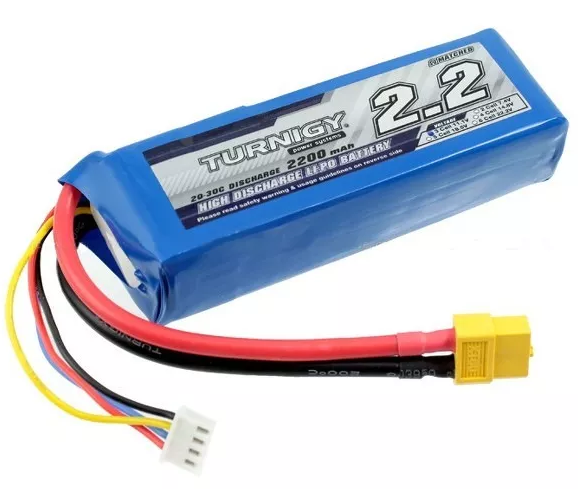
\includegraphics[scale=0.5]{Metodologia/Bateria2200}
    \caption{Bateria Lipo de duas células (7.4 $V_{cc}$) com capacidade de 2200 $mAh$ e taxa de carga e descarga 20 $C$.}
    \label{fig:Bateria2200}
\end{figure}

Com relação ao tempo de funcionamento, basta conhecer o valor de consumo de cada dispositivo que compõe o sistema. Para esse projeto, pode-se considerar apenas o consumo dos motores, Tabela (\ref{tab:ConsumoMotores}), já que a corrente drenada pelos outros eletrônicos são irrelevantes perante aos atuadores. Em teoria e considerando tudo em perfeitas condições, é possível obter 1 (uma) hora de funcionamento utilizando o torque máximo ou 110 min usando a máxima eficiência dos motores em descarga contínua. 
\begin{table}[!htb]
\centering
\caption{Consumo dos Motores CC.}
\label{tab:ConsumoMotores}
\begin{tabular}{@{}lcc@{}}
\toprule
\multicolumn{1}{c}{\textbf{Dispositivo}} & \textbf{Máx. Eficiência} & \textbf{Máx. Torque} \\ \midrule
Motores                          & 1.2 A                     & 2.2 A                 \\ \bottomrule
\end{tabular}
\end{table}

\subsection{Representação da Montagem do Circuito Eletrônico}

A representação esquemática do circuito eletrônico contendo todos os componentes detalhados aqui neste capítulo, pode ser visto na Figura (\ref{fig:circuitoEletronicoPlanta}). Pode-se observar através da figura como os componentes foram interligados uns aos outros. Essa é a representação final do circuito eletrônico para controle da posição angular da estrutura com a vertical.

\begin{figure}[H]
\centering
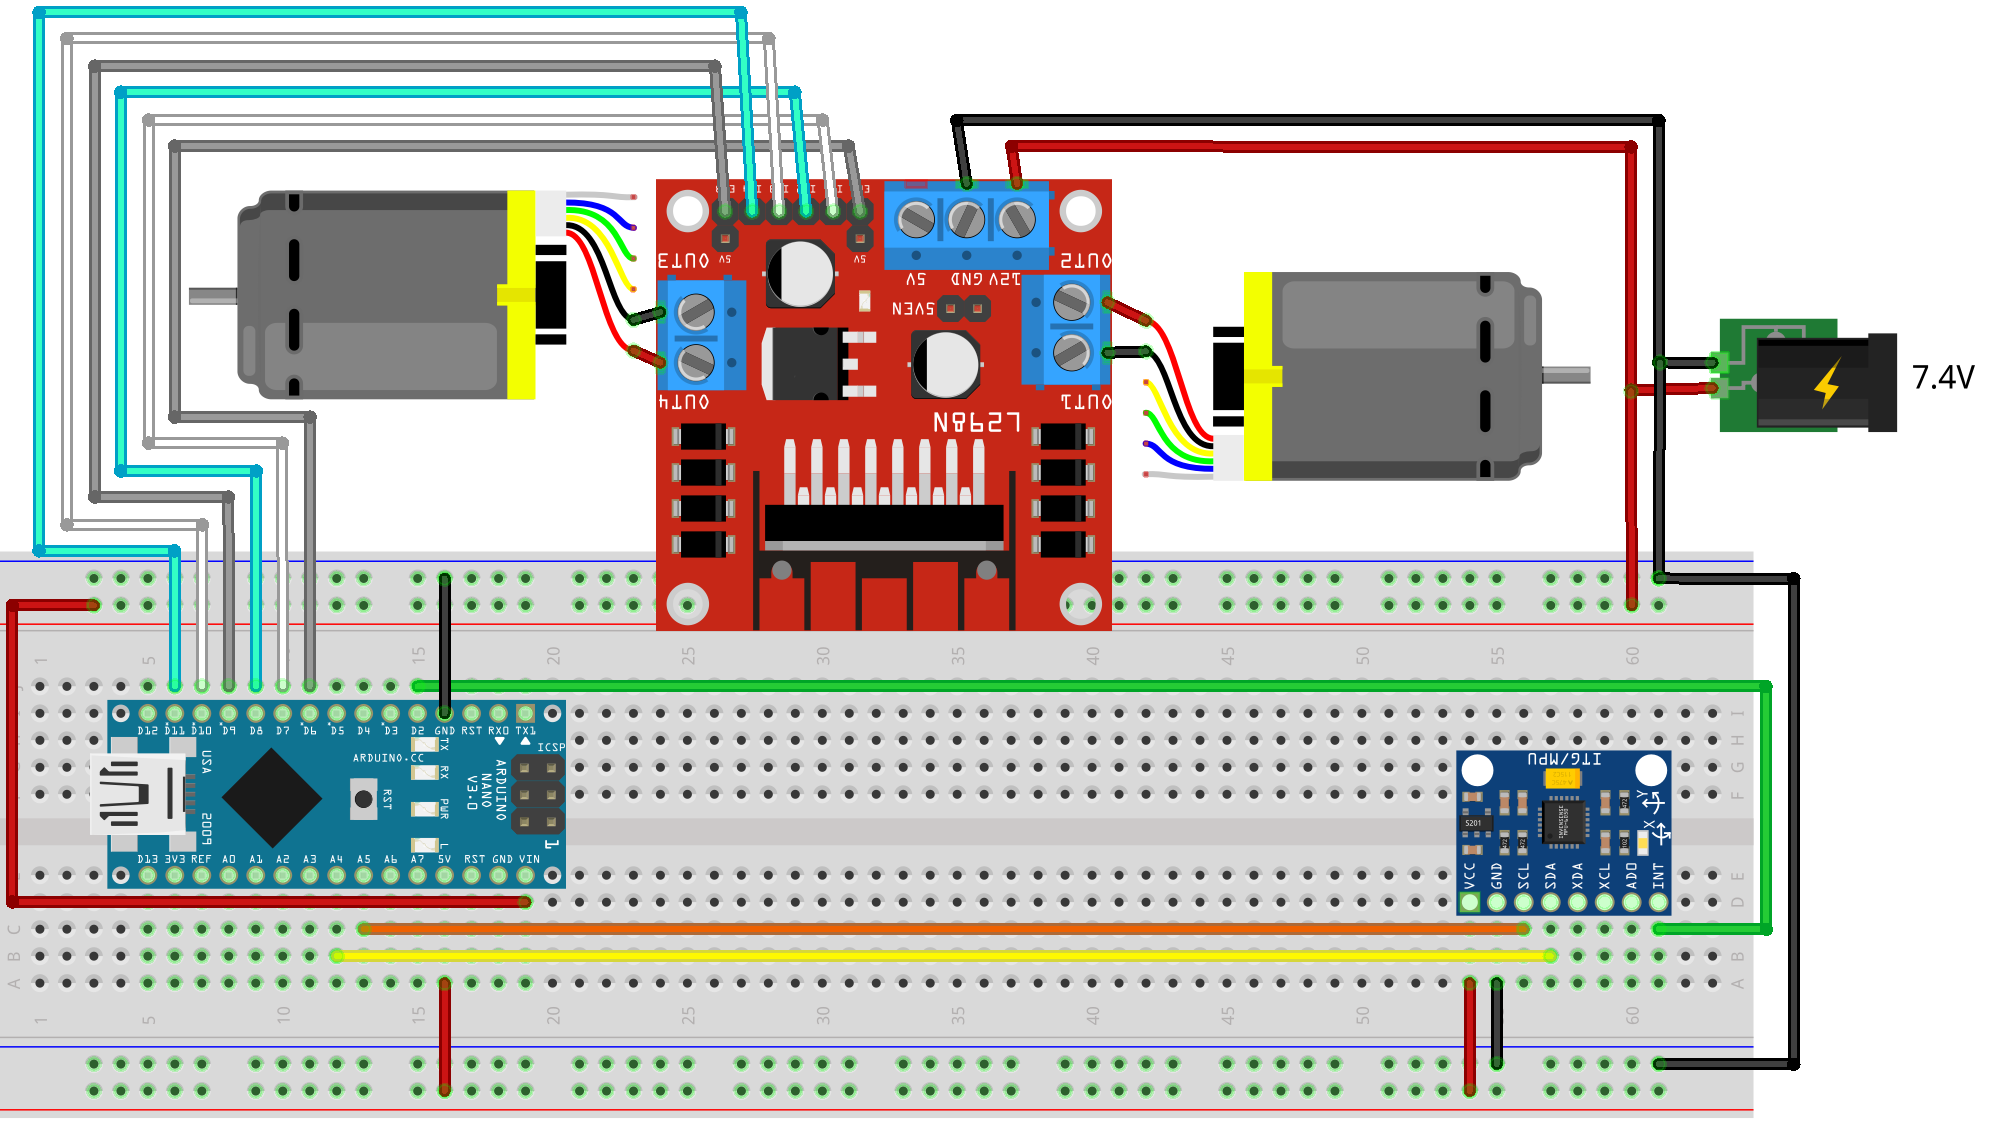
\includegraphics[width=16cm]{Resultados/CircuitoEletronico.png}
\caption{Representação do circuito eletrônico montado para controle da posição angular do pêndulo.}
\label{fig:circuitoEletronicoPlanta}
\end{figure}

\section{\textit{Softwares}}

A realização deste trabalho se deu através de uso de alguns \textit{softwares} que ajudaram e facilitaram bastante. Abaixo é feito um breve resumo de cada um e para qual propósito os mesmos serviram.

\subsection{SolidWorks}

O SolidWorks é um \textit{software} de CAD 3D, utilizado para modelagem de peças sólidas e para simulações de processos. Foi escolhido como plataforma para o desenvolvimento do projeto mecânico das peças da estrutura devido à experiência do autor com o programa, adquirido ao longo do curso.

\subsection{MATLAB}

O MATLAB é um \textit{software} interativo de alta performance voltado para o cálculo numérico. Realiza a análise numérica, cálculo com matrizes, processamento de sinais e construção de gráficos em ambiente fácil, sendo programado com linguagem matemática ao invés da programação tradicional. O \textit{software} conta com inúmeras extensões, mas com destaque para o Simulink. Essa extensão conta com uma programação baseada em diagrama de blocos e com esse \textit{toolbox} é possível realizar as simulações dos circuitos de uma forma que fique mais simples e de fácil visualização. Foi escolhido para realização dos cálculos de parâmetros mecânicos, dos ganhos do controlador e simulação do sistema.

\subsection{Arduino IDE}

É um \textit{software} gratuito, de código aberto, que facilita a gravação dos programas desenvolvidos na placa Arduino. A linguagem de programação é baseada em C. Foi utilizado no desenvolvimento do código responsável por acionar os motores de corrente contínua e também o processamento do controlador.

\subsection{Processing}

O Processing por sua vez é uma linguagem de programação de código aberto e possui um ambiente de desenvolvimento integrado (IDE). Contudo, ele é considerado um \textit{sketchbook}, alternativa de organização de projetos sem ser o de um IDE padrão. Por mais que seja baseado na linguagem Java, a forma de programar não é de Java puro, a não ser que o usuário deseja. Foi utilizado neste trabalho em conjunto com o Arduino para validação dos sinais do sensor, lendo dados através da porta serial do computador.

\subsection{Visual Studio Code (VS Code)}

O Visual Studio Code, ou popularmente conhecido como VS Code, é um editor de código-fonte desenvolvido pela Microsoft para Windows, Linux e macOS. É customizável, permitindo que os usuários possam mudar o tema do editor, teclas de atalho e preferências. É um \textit{software} livre e de código aberto. Foi utilizado para ler os sinais gravados em arquivo com extensão .txt do Processing utilizando linguagem python.

\subsection{\textit{Fritizing}}

O \textit{Fritizing} é uma iniciativa de código aberto para desenvolver um \textit{software} tipo CAD para desenhos de \textit{hardware} eletrônico, com intuito de apoiar a construção de um circuito mais permanente como a confecção de uma placa de circuito impresso (PCB). Utilizou desse \textit{software} para a elaboração de uma visão esquemática do circuito eletrônico da planta.

\section{Custo dos Materiais Adquiridos}

A seguir, na Tabela (\ref{tab:CustoMateriais}), estão listados os materiais utilizados para a elaboração mecânica e eletrônica do projeto, seus respectivos preços e a quantidade necessária.
\begin{table}[!htb]
\centering
\caption{Tabela de custo dos materiais utilizados na construção do protótipo.}
\label{tab:CustoMateriais}
\begin{tabular}{@{}lccccccc@{}}
\toprule
\multicolumn{1}{c}{\textbf{Descrição}} & \textbf{Un.} & \textbf{Qtd.} & \textbf{Valor Un.} & \textbf{Valor Total}  \\ \midrule
Arduino Nano            & pç  & 1   & R\$ 19,50   & R\$ 19,50   &                          \\
Kit Motor CC            & pç  & 2   & R\$ 119,90  & R\$ 239,80  &                          \\
Driver L298 H           & pç  & 1   & R\$ 19,90   & R\$ 19,90   &                          \\
MPU6050                 & pç  & 1   & R\$ 16,90   & R\$ 16,90   &                          \\
Bateria Lipo 2200mAh    & pç  & 1   & R\$ 130,00  & R\$ 130,00  &                          \\
Carregador Lipo Imax B6 & pç  & 1   & R\$ 110,00  & R\$ 110,00  &                          \\
Estrutura               & -   & 1   & R\$ 45,00   & R\$ 45,00   &                          \\
Miscelaneas             & -   & 1   & R\$ 58,00   & R\$ 58,00   &                           \\
\multicolumn{4}{l}{\textbf{TOTAL}}                                                       & \multicolumn{1}{l}{\textbf{R\$ 639,10}} \\ \bottomrule
\end{tabular}
\end{table}

O item denominado de miscelâneas da lista de materiais remete aos materiais que são difíceis de contar um a um e na maioria da vezes são parafusos, porcas, \textit{jumpers}, etc. Para encontrar seu valor, considerou-se 10\% do valor total de toda a lista.